\NOTE{REVISAR GRAMÁTICA Y ORTOGRAFÍA A PARTIR DE AQUÍ!!}
\subsection{Fase 2: Metaheurística de optimización multiobjetivo} \label{sec:3:metaheurística}
Se trata del núcleo principal del presente proyecto, pues trata de dar solución al problema en sí mediante un enfoque de metaheurísticas.

Como ya se ha introducido previamente, estamos ante un problema de \textit{timetabling/scheduling} que son generalmente problemas complejos debido a su naturaleza combinatoria. 
Matemáticamente se dice que pertenecen al conjunto de los problemas llamados \textit{NP-Duros (NP-Hard)}, pues los algoritmos clásicos empleados para resolverlos tienen una complejidad al menos de tipo exponencial.
Clásicamente se han empleado algoritmos para problemas concretos de este tipo que van desde el \textit{General Scheduling Problem} (GSP) que es el caso más general hasta los casos más concretos mediante variaciones respecto al anterior, haciéndolo más o menos restrictivo. 
Algunos son: el \textit{Open Shop Scheduling} (OSS), \textit{Job Shop Scheduling} (JSS), \textit{Flow Shop Scheduling} (FSS) o \textit{Permutational Flow Shop Scheduling} (PFSS). Una clasificación más detallada de este tipo de problemas clásicos se encuentra en~\cite{sota:tesis-doctoral}. 

Lejos del entorno académico, los problemas reales de \textit{scheduling} (como el que tenemos entre manos en esta tesis) pueden ser muy diferentes entre sí, habiendo pues mucha variedad en función del ámbito de aplicación. 
Por ejemplo se han estudiado casos para transporte público~\cite{sota:transporte-publico} o universidades~\cite{sota:universidad} y podemos ver cómo son completamente diferentes en cuanto a restricciones y necesidades de cada una de las soluciones, por lo que las metodologías empleadas para su resolución son bien diferentes.

Existen gran cantidad de técnicas que se han empleado previamente para resolver este tipo de problemas, comenzando por sencillos heurísticos aplicados a los problemas clásicos bien estudiados y formalizados, pero como hemos puntualizado antes, este tipo de algoritmos solamente son aplicables a instancias pequeñas debido a la mencionada naturaleza no polinómica, por lo que no son útiles en problemas reales. Por otro lado, se ha analizado cómo transformar un problema de \textit{scheduling} en un problema de coloreado de grafos~\cite{sota:estudio-coloreado-grafos, sota:algotimo-coloreado-grafos} lo que nos permite emplear los algoritmos existentes para este tipo de problemas, entre los que podemos encontrar exactos y aproximados. También existen enfoques más modernos que emplean técnicas de \textit{Aprendizaje Automático} habitualmente combinados con metaheurísticas~\cite{sota:machine-learning-geneticos} y recientemente \textit{Hiperheurísticas} (como por ejemplo en~\cite{sota:hiperheuristicas}). En el libro~\cite{sota:libro-sota-scheduling} se encuentran explicadas de forma detallada todas estas técnicas aquí nombradas.

Por último, la técnica más empleada actualmente para resolver este tipo de problemas son las metaheurísticas: una familia de algoritmos de carácter genérico empleados como \textit{framework} para resolver un problema dado. Tienen dos características principales~\cite{sota:metaheuristicas}:

\begin{enumerate}
	\item En contraposición a los heurísticos, no dependen directamente del problema específico, únicamente han de ser adaptados parcialmente.
	\item Por definición son métodos de búsqueda aproximados, que tratan de combinar técnicas de exploración y explotación (véase \autoref{capitulo:3:busqueda-divers-intens}) para obtener la mejor solución posible dentro del espacio de búsqueda definido.
\end{enumerate}

Tienen dos conceptos básicos que conforman la clave para su implementación para un problema concreto: la función objetivo y la codificación. 

La codificación permite representar una solución de la forma más compacta posible sin perder información del dominio. Una buena codificación tendrá las siguientes características~\cite{sota:metaheuristicas-design-impl}:

\begin{itemize}
	\item Completitud: Todas las soluciones asociadas con el problema deben poder ser representadas. Se debe garantizar una representatividad total dentro del espacio de soluciones: si no es definida correctamente podría haber soluciones incapaces de ser representadas y lógicamente afectará a la eficiencia de la metaheurística.
	\item Conectividad: Debe existir un camino que permita moverse entre dos soluciones del espacio de búsqueda, de forma que cualquier solución del espacio pueda ser alcanzada (en especial el optimo global).
	\item Eficiencia: Fácil de manipular por los operadores de la búsqueda (definidos por cada metaheurística).
\end{itemize}

Por su parte, la función objetivo o de evaluación (en inglés denominada \textit{fitness}) permite la comparación de soluciones entre sí y representará el objetivo de la búsqueda, de forma que si nos enfrentamos a un problema con varios parámetros objetivo, podamos ponderarlos u ordenarlos según los criterios que se adecuen al problema. Existen varios enfoques para definir una función de evaluación de un problema multiobjetivo: enfoques escalares, basados criterios, basados en dominaciones (óptimos de Pareto) entre las soluciones o basados en indicadores de calidad. Los más sencillos son los primeros, pues permiten trasformar el problema multiobjetivo en uniobjetivo y al ser el empleado en esta tesis será descrito con mayor detenimiento en el \autoref{apartado:adaptacion-VNS}

Por otro lado, las metaheurísticas emplean una o varias soluciones que son comparadas entre sí empleando una función de comparación o evaluación  que suele ser de un coste computacional importante. Ésta función será dependiente del problema a resolver.

Estas técnicas fueron muy innovadoras, pues permitieron la resolución de muchos problemas clásicos que hasta entonces no podían resolverse con técnicas clásicas. Además, soportan perfectamente instancias grandes, por lo que hasta la fecha es la técnica más prometedora para el problema a resolver en esta tesis.

No obstante, la mayor desventaja de las metaheurísticas es que, al tratarse de métodos aproximados, no garantizan que se encuentre una solución óptima global ni que se encuentre acotada en algún rango de valores~\cite{sota:metaheuristicas-design-impl} como sí permiten otras técnicas. Una pequeña desventaja frente a todas las posibilidades que las metaheurísticas nos ofrecen.
 
Una vez decidida la técnica a emplear para resolver el problema definido, el siguiente paso es elegir de entre el catálogo de metaheurísticas existentes hasta la fecha, una de ellas. A lo largo del tiempo se han ido proponiendo diferentes taxonomías para ordenar toda esta gran cantidad de metaheurísticas. 
Así, una de las clasificaciones más conocidas es la propuesta por Osman en~\cite{metaheuristicas:taxonomia1} que distingue entre aquellas basadas en búsquedas locales (pequeños cambios a una misma solución), las constructivas (en cada iteración se van añadiendo partes que al final conforman una solución al completo) y las poblacionales (se combinan varias soluciones entre sí). 

Gendreau y Potvin~\cite{metaheuristicas:taxonomia2} propusieron en 2005 una clasificación dicotómica: aquellas de tipo trayectorial y de tipo poblacional, combinando así las de búsqueda local y las constructivas en un mismo grupo que emplea unicamente una sola solución por iteración mientras que las segundas emplean un conjunto dinámico de soluciones que en cada iteración irá cambiando. 

Existen otras clasificaciones menos relevantes que dividen las metaheurísticas en aquellas inspiradas en la naturaleza y aquellas que no, en si emplean capacidad de memoria o no, o si son de naturaleza determinista o estocástica. Una de las últimas clasificaciones~\cite{sota:metaheuristicas} propone la división en metafóricas (metáforas de la biología, química, música, matemáticas, física o social-deportiva) o no metafóricas.

En el caso de este proyecto, la elección fue de carácter histórica: los proyectos previos habían empleado dos metaheurísticas y una de ellas parecía dar resultados más prometedores que la otra. Estamos hablando de la metaheurística \textit{Variable Neighborhood Search} (\textit{Búsqueda de Entornos Variable}) que describiremos en las próximas secciones y veremos cómo ha sido adaptada a nuestro problema.

\subsubsection{Búsqueda en Entornos Variables (VNS)}
Se trata de una metaheurística trayectorial, pues maneja una única solución en cada iteración, además de tipo búsqueda local pues trata de modificarla iterativamente para mejorarla empleando un catálogo de \textit{entornos} o vecindades (\textit{neighborhoods}). A su vez es de tipo no metafórica: no se inspira en ningún proceso de la naturaleza. Es además de tipo estocástico y no emplea memoria para su funcionamiento.

Su nombre radica precisamente en sus dos conceptos fundamentales: búsqueda local y entornos variables. Se fundamenta en dos etapas~\cite{vns}: descenso y perturbación, la primera consiste en el intercambio sistemático del entorno empleado durante una búsqueda local simple que nos permite alcanzar un óptimo local; mientras que la segunda radica en la alteración aleatoria de la solución para evitar atascarse en óptimos locales evitando así una convergencia prematura.

Así pues, el VNS parte de una lista predefinida de entornos, que definen el criterio a emplear para moverse entre soluciones a partir de una inicial. Al entorno $k$ del conjunto de vecindades se les suele denotar como $N_k, k=1,...,k_{max}$ y al conjunto de soluciones alcanzables mediante la vecindad $k$ como $N_k(x)$.
Un ejemplo sencillo de entorno podría ser en el caso de una optimización de una variable en el dominio $\mathbb{R}$: un posible entorno sería $N_1=[x-2, x+2]$ o $N_2=[x-7, x+7]$, ilustrados en la \autoref{fig:ejemplos-entorno}.

\begin{figure}[htbp]
	\centering
	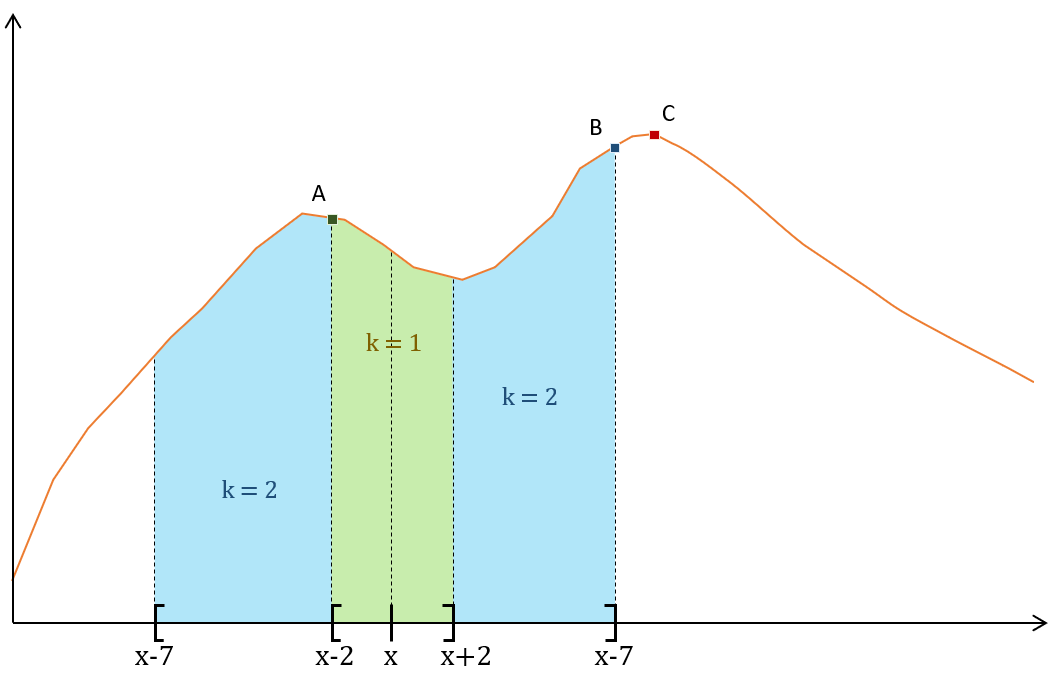
\includegraphics[width=\linewidth]{ejemplos-entorno}
	\caption{Ejemplo de dos entornos definidos en $\mathbb{R}$}
	\label{fig:ejemplos-entorno}
\end{figure}

Como podemos observar, los entornos se definen con respecto a una solución, denotada por $x$. En el ejemplo los entornos se han definido de forma que el conjunto de soluciones alcanzables mediante el segundo sea un superconjunto del aquel empleando el primero, ampliando de esta forma las fronteras de la búsqueda (no es necesario definirlos así pero suele ser una práctica habitual). Si lanzamos una búsqueda local sobre la función del ejemplo empleando el entorno $k_1$, el punto más optimo que podemos alcanzar en caso de maximización es el punto $A$, mientras que si empleamos el $k_2$ será el $B$. El punto $C$ es el óptimo global de la función, que no es alcanzado por ninguno de los entornos definidos, aunque $k_2$ se aproxima bastante. 

No necesariamente un entorno amplio, i.e. con mayor conjunto de soluciones factibles, es mejor que uno más reducido, pues el espacio de búsqueda es mayor y esto repercutirá decisivamente en el rendimiento del algoritmo de búsqueda. Además, en problemas más complejos con un mayor número de variables, el espacio de búsqueda es mucho más complejo y difícil de explorar.

Con todo, el VNS se basa en tres caraterísticas:

\begin{enumerate}
	\item Un óptimo local respecto a una estructura de vecindad no necesariamente lo es respecto a otra.
	\item Un óptimo global es a su vez óptimo local respecto a todas las posibles estructuras de entornos.
	\item Empíricamente se ha determinado que para la mayoría de problemas, los óptimos locales con la misma o distinta estructura de entornos están relativamente cerca.
\end{enumerate}

En la \autoref{fig:VNS-facts} se ilustran estas tres características visualmente.

\begin{figure}[htbp]
	\centering
	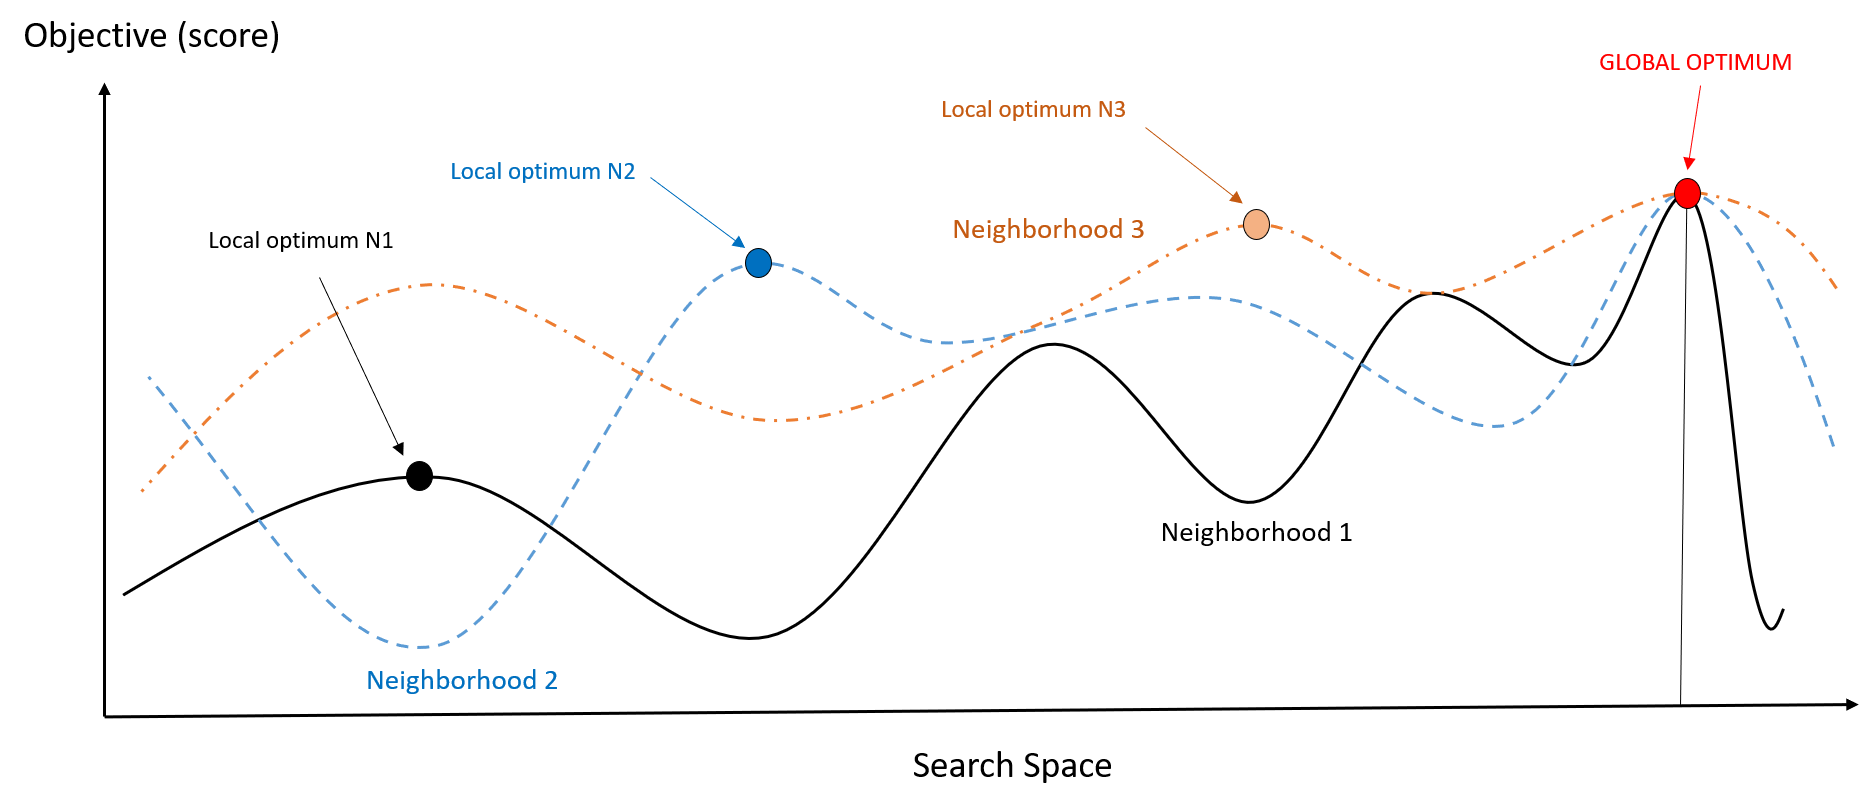
\includegraphics[width=\linewidth]{VNS-facts}
	\caption[Ilustración que representa las características sobre las que se fundamenta el VNS]{Ilustración que representa las características sobre las que se fundamenta el VNS. Imagen proporcionada por Adolfo Urrutia Zambrana}
	\label{fig:VNS-facts}
\end{figure}

Comenzaremos analizando el cambio entre entornos, que se lleva a cabo de la misma forma en todo VNS siguiendo el \autoref{algoritmo:VNS-cambio-entornos}. 
Como se puede observar, se llevan a cabo acciones diferentes en función de si la nueva solución obtenida por el algoritmo de búsqueda local es mejor que la de partida. La función fitness se ha denotado como $f(x) \in [0,1]$


\begin{algorithm}[htbp]
	%	\SetAlgoLined
	\DontPrintSemicolon
	\KwData{
		
		$x$, solución actual. En la primera iteración es la inicial.
				
		$x'$, solución obtenida del algoritmo de búsqueda local con el entorno $k$
		
		$k$, indice de la vecindad actual
	}
	\medskip

	\If{$f(x')>f(x)$}{
		$x \leftarrow x'$  [Moverse a la mejor solucion] \;
		$k \leftarrow 1$  [Reinicio de vecindades] \;
	}
	\Else{
		$k \leftarrow k+1$  [Siguiente vecino] \;
	}
	
	\caption{Algoritmo del VNS empleado para el cambio de vecindades en caso de un problema de maximización}
	\label{algoritmo:VNS-cambio-entornos}
\end{algorithm}

En cuanto al comportamiento de la búsqueda, el VNS en su versión básica (conocido como \textit{Basic VNS}) se compone de dos fases: la búsqueda local y la ``agitación`` (\textit{shake}) siendo la primera determinista y la segunda estocástica. Una componente aleatoria aporta nueva información a la búsqueda que podría ser de ayuda a la componente determinista.

La componente de búsqueda local se puede realizar en dos enfoques diferentes: buscando la primera solución que mejore la actual (\textit{First Improvement}) o empleando la mejor de todas las posibles soluciones del entorno (\textit{Best Improvement}) sin embargo no siempre es posible obtener todas las soluciones posibles de un entorno, especialmente en problemas complejos como el que tenemos entre manos. En éste problema se ha empleado una técnica mixta que si bien no emplea la mejor solución, tampoco emplea la primera mejor, sino que continúa la búsqueda hasta que la solución no se mejore en un porcentaje de tolerancia (véase \NOTE{REFERENCIA} para una descripción detallada). %TODO REFERENCIA!!

Los algoritmos \ref{algoritmo:BestImprovement} y \ref{algoritmo:FirstImprovement} se han obtenido directamente de Hansel et al. \cite{vns} y describen el proceso asociado al \textit{Best Improvement} y al \textit{First Improvement}. respectivamente

\begin{algorithm}[htbp]
%	\SetAlgoLined
\DontPrintSemicolon
\KwData{
$x$, solución actual.
}
\medskip

\Repeat{
	$f(x) \le f(x')$
}{
	$x' \leftarrow x$ \;
	$x \leftarrow \arg \max_{y \in N(x')} f(y)$ \;
}
\Return x \;

\caption{Best Improvement}
\label{algoritmo:BestImprovement}
\end{algorithm}

\begin{algorithm}[htbp]
	%	\SetAlgoLined
	\DontPrintSemicolon
	\KwData{
		$x$, solución actual. 
	}
	\medskip
	
	\Repeat{
		$f(x) \le f(x')$
	}{
		$x' \leftarrow x$ \; 
		$i \leftarrow 0$ \;
		\Repeat{$f(x) > f(x')$ ó $i = |N(x)|$}{
			$i \leftarrow i + 1$ \;
			$x \leftarrow \arg \max \left\lbrace f(x), f(x^i)\right\rbrace $, $x^i \in N(x)$ \;
		}
	}
	\Return x \;
	
	\caption{First Improvement}
	\label{algoritmo:FirstImprovement}
\end{algorithm}

Por el otro lado, la componente estocástica introduce en la búsqueda una solución generada de forma aleatoria, de manera que nueva información se introduce en el proceso de búsqueda que puede mejorar el valor de fitness empleando, por ejemplo fragmentos de aleatoria que de forma determinista nunca podrían haberse logrado o como mínimo habría sido necesario un mayor tiempo de cómputo. En el \autoref{algoritmo:Basic-VNS} se muestra el proceso esquemáticamente para el VNS Básico. Nótese que la condición de parada es únicamente el tiempo de cómputo, no obstante, se suele combinar con un porcentaje mínimo de mejoría de forma que si la búsqueda se estanca, no se pierda tiempo de cómputo innecesariamente. Las condiciones de parada del algoritmo se encuentran descritas en profundidad en la \autoref{apartado:condiciones-parada}.

\begin{algorithm}[htbp]
	%	\SetAlgoLined
	\DontPrintSemicolon
	\KwData{
		
		$x$, solución actual. 
		
		$k_{max}$, número de entornos definidos para la metaheurística.
		
		$t_{max}$, tiempo máximo de ejecución del algoritmo.
	}

%	\medskip
	\bigskip
	
	$t \leftarrow 0$ \;
	
	\While{$t<t_{max}$}{
		
		\Repeat{
			$k = k_{max}$
		}{
			$x' \leftarrow \texttt{Shake}(x,k)$ [Componente estocástica]
			$x'' \leftarrow \texttt{FirstImprovement}(x')$ [Búsqueda local]
			$x,k \leftarrow \texttt{NeighbourhoodChange}(x,x'',k)$ [Cambio de vecindad]
		}
		$t \leftarrow \texttt{CpuTime}()$ [Medición del tiempo de ejecución]
	}

	\Return x \;
	
	\caption{Basic VNS \cite{vns}}
	\label{algoritmo:Basic-VNS}
	

\end{algorithm}

Por supuesto, cada problema es diferente y se adapta mejor a un método u otro y es por eso que con el tiempo se han definido algunas variaciones de VNS básico y que reciben nombres diferentes. La forma más sencilla de variar el método es suprimir una de las dos componentes: si sustituimos la componente estocástica, dejando la búsqueda únicamente determinista tenemos el \textit{Variable Neighborhood Descendent (VND)}; mientras que si la búsqueda es únicamente estocástica tenemos el \textit{Reduced Variable Neighborhood Search (RVNS)}. Éste último es el menos costoso computacionalmente, sin embargo es el que menos información del problema emplea y su rendimiento suele ser peor que los demás. 

Otra posible variación se basa en  emplear una técnica distinta para la búsqueda local. Si por ejemplo empleamos otro VNS únicamente determinista, es decir un VND (descendent) en lugar de una búsqueda local simple, estaremos empleando un \textit{General VNS}.

Por último, existen otras variaciones que rompen con la estructura básica del VNS pero que se ha visto que dan buenos resultados para ciertos problemas,  mejorando las variaciones anteriores. Entre ellas, el \textit{Skewed VNS} (SVNS) definido en \cite{svsn-def} cuya idea se basa en explorar óptimos locales lejanos a óptimo actual, potenciando la exploración sobre la explotación intrínseca al propio VNS por definición. Así, podrá moverse entre soluciones peores con el fin de encontrar información reutilizable en la solución, sin embargo, la exploración de debe realizarse demasiado lejos de la solución actual, pues podría degenerar en una búsqueda de inicio múltiple (\textit{multistart}), donde se hacen búsquedas repetidamente empleando como solución de inicio una generada aleatoriamente, y ésto se sabe que es ineficiente para este tipo de problemas \cite{vns}). Para evitar ésto, se define una función de distancia de forma que si la solución peor a explorar está demasiado lejos de la actual, se descarte.

Para ello, el SVNS define un parámetro adicional denotado normalmente como $\alpha$, que multiplica la función de distancia y es el que permite la exploración más o menos lejos de la solución actual. El \autoref{algoritmo:VNS-cambio-entornos} se redefine de la siguiente manera:

\begin{algorithm}[h]
	%	\SetAlgoLined
	\DontPrintSemicolon
	\KwData{
		
		$x$, solución actual. En la primera iteración es la inicial.
		
		$x'$, solución obtenida del algoritmo de búsqueda local con el entorno $k$
		
		$k$, indice de la vecindad actual
		
		$\alpha$, parámetro de la metaheurística
	}
	\bigskip
	
	\If{$f(x')+\alpha \cdot \rho(x,x') > f(x)$}{
		$x \leftarrow x'$  [Moverse a la mejor solucion] \;
		$k \leftarrow 1$  [Reinicio de vecindades] \;
	}
	\Else{
		$k \leftarrow k+1$  [Siguiente vecindad] \;
	}
	
	\caption{Redefinición del algoritmo de cambio de vecindades para un \textit{Skewed} VNS en un problema de maximización}
	\label{algoritmo:SVNS-cambio-entornos}
\end{algorithm}

Donde $\rho(x,x')$ es la función de distancia definida para el problema concreto.

El algoritmo central del SVNS es homólogo al \autoref{algoritmo:Basic-VNS} con la diferencia de que debido a que el nuevo algoritmo de cambio de entorno no retorna la mejor solución, sino la próxima a explorar (de peor \textit{fitness} pero alejada de ella), debemos almacenar la mejor para no perderla, y actualizarla en cada iteración. Además, será la que devolvamos al final del algoritmo.

Existen más variaciones del algoritmo básico del VNS que no se han contemplado en éste proyecto, por lo que no se encuentran definidas aquí. Más información al respecto puede hallarse en \cite{vns} y \cite{info-adicional-vns}

\subsubsection{Adaptación del VNS al problema}
\label{apartado:adaptacion-VNS}

Una vez definida la técnica a utilizar y las posibles variaciones planteadas, debemos instanciar los parámetros del algoritmo y definir las heurísticas ---dependientes del problema concreto--- necesarias de la metaheurística.

En las próximas secciones se describe cómo se ha optado por adaptar la metaheurística descrita en la sección anterior al problema descrito en el \autoref{capitulo:2}: cómo se ha implementado la función de evaluación, qué entornos se han definido y bajo qué criterios son ordenados, las técnicas de exploración y explotación utilizadas y, finalmente, las condiciones de parada

La primera característica necesaria para las metaheurísticas ---y cualquier técnica, en palabras generales--- es la codificación (definida en la sección anterior). En el caso de nuestro problema, tal y como se describió detalladamente en la \autoref{apartado:representacion-soluciones}, las soluciones se representan de forma matricial con una discretización del tiempo a intervalos de 5 minutos. La representación desde el punto de vista de la programación se encuentra descrita en la \autoref{sec:detalles-impl-sistema}. % TODO ajustar referencia cruzada

\paragraph{Función Fitness} 
La función fitness tiene por objeto la evaluación de una solución de manera que se puedan comparar entre sí dos o más soluciones del problema y poder decidir cuál es la mejor.  Para poder definir una función de evaluación hacen falta uno o más \textit{objetivos} o \textit{criterios}. En caso de encontrar un único objetivo estaremos ante una búsqueda \textit{uniobjetivo}, mientras que si hay varios, sería \textit{multiobjetivo} o \textit{multicriterio}. En los problemas reales es habitual encontrarse con más de un criterio, algunos quizás contradictorios entre sí, por lo que aparece la figura del \textit{decisor}, que suele ser el cliente o el principal stakeholder del proyecto, y es el encargado de seleccionar aquellos objetivos que considere más relevantes (e incluso ponderarlos si es preciso) de esta forma se resuelven los conflictos entre objetivos. Otra opción para resolver ésto consiste en presentar al decisor un conjunto de soluciones y que este elija la que más le convenga en función de sus criterios. En nuestro caso, si bien podríamos haber optado por cualquiera de las dos decisiones, por razones históricas, se empleó la primera opción. 

Nuestro decisor, los responsables del proyecto por parte de \gls{CRIDA}, % TODO: Poner nombres???
 deberá ponderar los objetivos según sus criterios. En éste caso, \gls{CRIDA} aún no ha ponderado los objetivos, por lo que se utilizó una técnica




Como se ha descrito previamente en la \autoref{sec:3:metaheurística}, en caso de una optimización multio



\paragraph{Definiciones de entornos}
Lorem ipsum

\paragraph{Búsqueda diversificada/intensificada} \label{capitulo:3:busqueda-divers-intens}
Lorem ipsum

\paragraph{Condiciones de Parada}
\label{apartado:condiciones-parada}
Lorem ipsum










